\documentclass[sigconf,nonacm]{acmart}

%% Enable subfigures
\usepackage{subfigure}
%% Enable numbers in scientific format.
\usepackage{siunitx}
%% Enable enumerate start from.
\usepackage{enumitem}

%% Enable theorems
\newtheorem{theorem}{Theorem}[section]
\newtheorem{lemma}[theorem]{Lemma}

%% Enable algorithms
\usepackage{algorithm}
\usepackage[noend]{algpseudocode}
\let\ReturnInline\Return
\renewcommand{\Return}{\State\ReturnInline}
\algrenewcommand\algorithmicrequire{$\rhd$}
\algrenewcommand\algorithmicensure{$\square$}

%% Fonts used in the template cannot be substituted; margin 
%% adjustments are not allowed.
\AtBeginDocument{%
  \providecommand\BibTeX{{%
    \normalfont B\kern-0.5em{\scshape i\kern-0.25em b}\kern-0.8em\TeX}}}

%% Rights management information.
\setcopyright{acmcopyright}
\copyrightyear{2018}
\acmYear{2018}
\acmDOI{XXXXXXX.XXXXXXX}

%% These commands are for a PROCEEDINGS abstract or paper.
\acmConference[Conference acronym 'XX]{Make sure to enter the correct
  conference title from your rights confirmation emai}{June 03--05,
  2018}{Woodstock, NY}
%% Title of the proceedings is different from ``Proceedings of ...''?
% \acmBooktitle{Woodstock '18: ACM Symposium on Neural Gaze Detection,
%  June 03--05, 2018, Woodstock, NY} 
% \acmPrice{15.00}
% \acmISBN{978-1-4503-XXXX-X/18/06}

%% Submission ID.
% \acmSubmissionID{123-A56-BU3}

%% Use the "author year" style of citations and references?
% \citestyle{acmauthoryear}

%% Message
\newcommand{\kk}[1]{{{\color{red} #1}}}
\newcommand{\ds}[1]{{{\color{blue} #1}}}
\newcommand{\su}[1]{{{\color{green} #1}}}

%% Ignore block
\newcommand{\ignore}[1]{}

%% Macros
\newcommand{\Lou}{\textit{Louvain}}
\newcommand{\LPA}{\textit{LPA}}
\newcommand{\Hyb}{\textit{Hybrid Louvain-LPA}}
\newcommand{\Sta}{\textit{Static}}
\newcommand{\Nai}{P-ND}
\newcommand{\DelOrg}{\textit{$\Delta$-screening}}
\newcommand{\Del}{P-DDS}
\newcommand{\Fro}{P-DF}
\newcommand{\StaLou}{\textit{Static Louvain}}
\newcommand{\NaiLou}{$\text{P-ND}_\text{L}$}
\newcommand{\DelLou}{$\text{P-DDS}_\text{L}$}
\newcommand{\FroLou}{$\text{P-DF}_\text{L}$}
\newcommand{\StaLPA}{\textit{Static LPA}}
\newcommand{\NaiLPA}{$\text{P-ND}_\text{LPA}$}
\newcommand{\DelLPA}{$\text{P-DDS}_\text{LPA}$}
\newcommand{\FroLPA}{$\text{P-DF}_\text{LPA}$}
\newcommand{\FroHyb}{$\text{P-DF}_\text{H}$}




\begin{document}

%% Full title of the paper.
\title{Heuristics for Inequality minimization in PageRank values}

%% Short title to be used in page headers (optional).
% \title[short title]{full title}
% \subtitle{Something other than the title}

%% Authors and their affiliations.
\author{Subhajit Sahu}
\email{subhajit.sahu@research.iiit.ac.in}
\affiliation{%
  \institution{IIIT Hyderabad}
  \streetaddress{Professor CR Rao Rd, Gachibowli}
  \city{Hyderabad}
  \state{Telangana}
  \country{India}
  \postcode{500032}
}

%% Concise author list in page headers.
%\renewcommand{\shortauthors}{Sahu, Kothapalli, and Banerjee, et al.}

%% Show page numbers.
\settopmatter{printfolios=true}

%% Short summary of the work to be presented in the article.
\begin{abstract}
This research study investigates the minimization of inequality in the ranks of vertices obtained using the PageRank algorithm. PageRank is a widely used algorithm for ranking webpages and plays a significant role in determining web traffic. This study employs the Gini coefficient, a measure of income/wealth inequality, to assess the inequality in PageRank distributions on various types of graphs. The investigation involves two experiments: one that modifies strategies for handling dead-end nodes and another that explores six deterministic methods for reducing inequality. Our findings indicate that a combination of two distinct heuristics may present an effective strategy for minimizing inequality.
\end{abstract}

%% The code below is generated by the tool at http://dl.acm.org/ccs.cfm.
\begin{CCSXML}
<ccs2012>
<concept>
<concept_id>10003752.10003809.10003635</concept_id>
<concept_desc>Theory of computation~Graph algorithms analysis</concept_desc>
<concept_significance>500</concept_significance>
</concept>
</ccs2012>
\end{CCSXML}

\ccsdesc[500]{Theory of computation~Graph algorithms analysis}

%% Pick words that accurately describe the work being presented.
\keywords{PageRank algorithm, Inequality minimization heuristics}

% \received{20 February 2007}
% \received[revised]{12 March 2009}
% \received[accepted]{5 June 2009}



%% Process the author and title information.
\maketitle

\section{Introduction}
\label{sec:introduction}
The PageRank algorithm is a critical tool in web search and ranking, determining the order of search results on popular search engines. This algorithm evaluates webpages' popularity based on the idea that pages linked by other popular pages are themselves considered popular. This can result in a positive feedback loop, where already popular pages receive even more traffic, exacerbating inequality.

Inequality in web ranking is a pressing concern, as excessive inequality can lead to social unrest. To address this issue, this research focuses on minimizing inequality in PageRank rankings using various heuristics. Two main experiments are conducted: adjusting dead-end handling strategies and comparing deterministic approaches for inequality minimization.




%% - Use --- for a dash.
%% - Use ``camera-ready'' for quotes.
%% - Use {\itshape very} or \textit{very} for italicized text.
%% - Use \verb|acmart| or {\verb|acmart|} for mono-spaced text.
%% - Use \url{https://capitalizemytitle.com/} for URLs.
%% - Use {\bfseries Do not modify this document.} for important boldface details.
%% - Use \ref{fig:name} for referencing.

%% For a block of pre-formatted text: 
% \begin{verbatim}
%   \renewcommand{\shortauthors}{McCartney, et al.}
% \end{verbatim}

%% For a list of items:
% \begin{itemize}
% \item the ``ACM Reference Format'' text on the first page.
% \item the ``rights management'' text on the first page.
% \item the conference information in the page header(s).
% \end{itemize}

%% For a table:
% \begin{table}
%   \caption{Frequency of Special Characters}
%   \label{tab:freq}
%   \begin{tabular}{ccl}
%     \toprule
%     Non-English or Math&Frequency&Comments\\
%     \midrule
%     \O & 1 in 1,000& For Swedish names\\
%     $\pi$ & 1 in 5& Common in math\\
%     \$ & 4 in 5 & Used in business\\
%     $\Psi^2_1$ & 1 in 40,000& Unexplained usage\\
%   \bottomrule
% \end{tabular}
% \end{table}

%% For a full-width table:
% \begin{table*}
%   \caption{Some Typical Commands}
%   \label{tab:commands}
%   \begin{tabular}{ccl}
%     \toprule
%     Command &A Number & Comments\\
%     \midrule
%     \texttt{{\char'134}author} & 100& Author \\
%     \texttt{{\char'134}table}& 300 & For tables\\
%     \texttt{{\char'134}table*}& 400& For wider tables\\
%     \bottomrule
%   \end{tabular}
% \end{table*}


%% For inline math:
% \begin{math}
%   \lim_{n\rightarrow \infty}x=0
% \end{math},

%% For a numbered equation:
% \begin{equation}
%   \lim_{n\rightarrow \infty}x=0
% \end{equation}

%% For an unnumbered equation:
% \begin{displaymath}
%   \sum_{i=0}^{\infty} x + 1
% \end{displaymath}

%% For a figure:
% \begin{figure}[h]
%   \centering
%   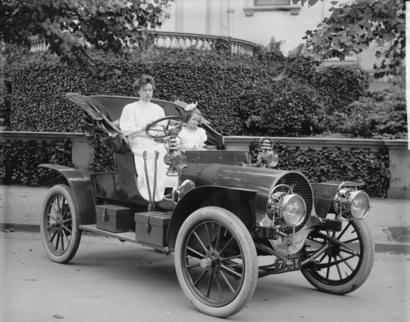
\includegraphics[width=\linewidth]{inc/sample-franklin}
%   \caption{1907 Franklin Model D roadster. Photograph by Harris \&
%     Ewing, Inc. [Public domain], via Wikimedia
%     Commons. (\url{https://goo.gl/VLCRBB}).}
%   \Description{A woman and a girl in white dresses sit in an open car.}
% \end{figure}

%% For a teaser figure.
% \begin{teaserfigure}
%   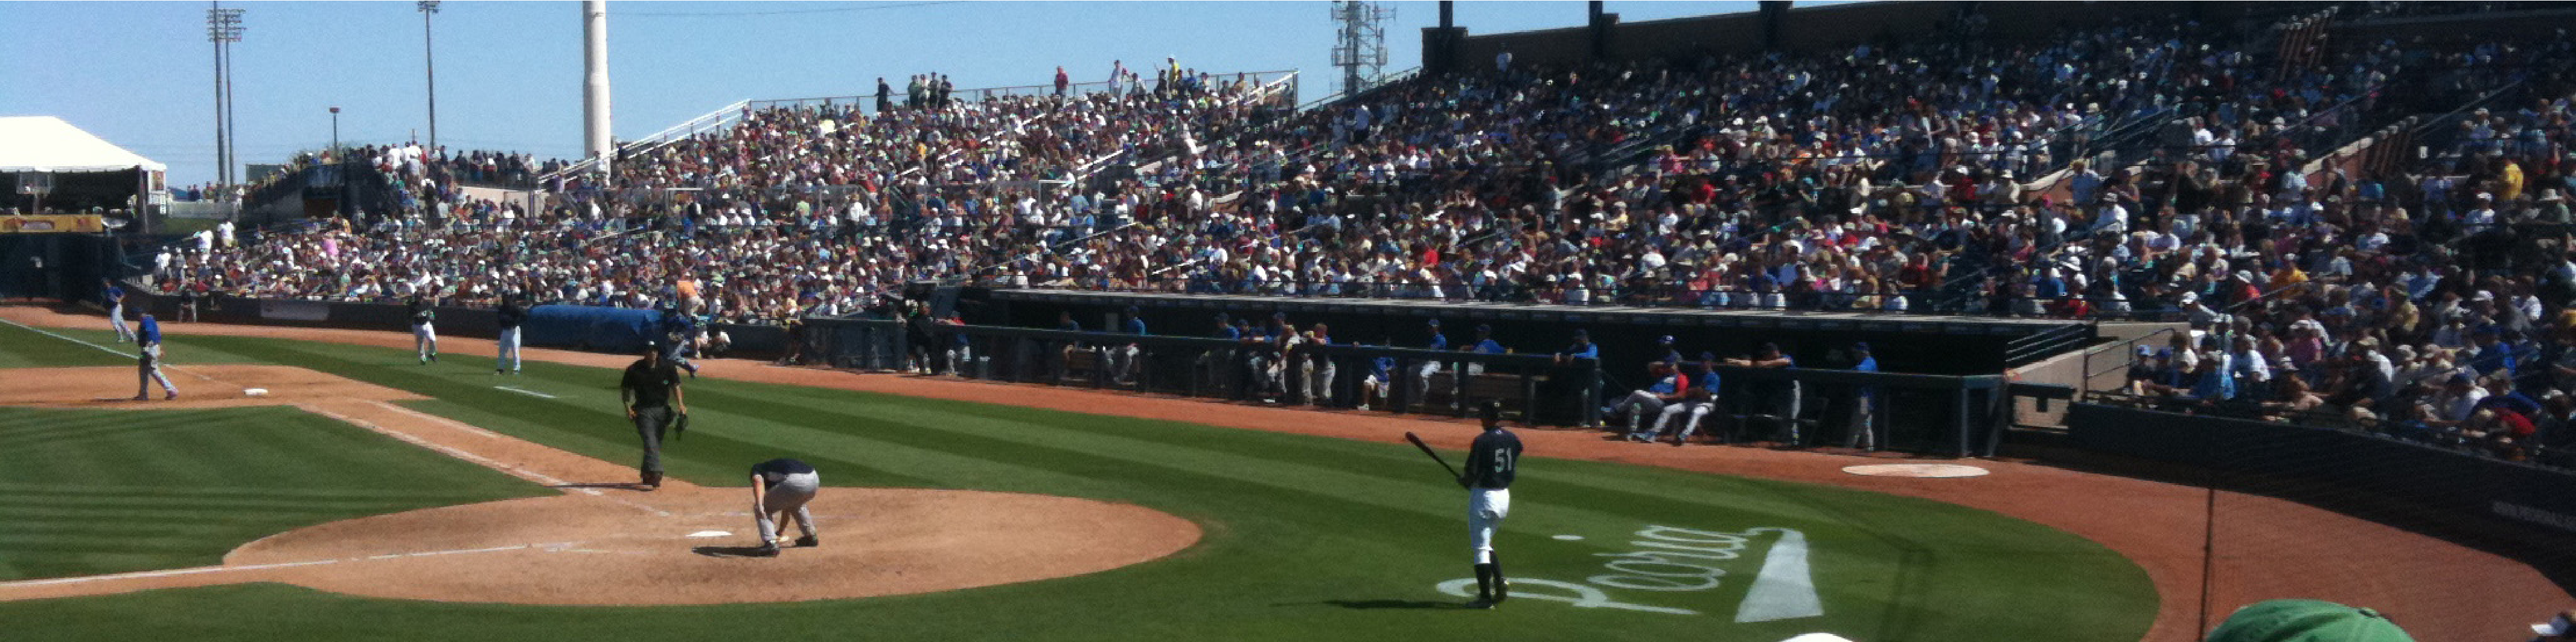
\includegraphics[width=\textwidth]{sampleteaser}
%   \caption{figure caption}
%   \Description{figure description}
% \end{teaserfigure}


\section{Related work}
\label{sec:related}
Algorithmic fairness has attracted significant attention in the past years \cite{tsioutsiouliklis2021fairness}. Given two groups of nodes, we say that a network is fair, if the nodes of the two groups hold equally central positions in the network \cite{pitoura2023pagerank}. Saxena et al. \cite{saxena2022fairsna} note that structural bias of social networks impact the fairness of a number of algorithms used for social-network analysis. Xie et al. \cite{xie2021fairrankvis} present a visual analysis framework for exploring multi-class bias in graph algorithms.

Tsioutsiouliklis et al. \cite{tsioutsiouliklis2021fairness} two classes of fair PageRank algorithms - fairness-sensitive PageRank and locally fair PageRank. They define a stronger fairness requirement, called universal personalized fairness, and show that locally fair algorithms also achieves this requirement. Krasanakis et al. \cite{krasanakis2021applying} present an algorithm for fair ranking with personalization, even when the personalization suffers from extreme bias while maintaining good rank quality. In another paper, Tsioutsiouliklis et al. \cite{tsioutsiouliklis2022link} provide formulae for estimating the role of existing edges in fairness, and for computing the effect of edge additions on fairness. They then propose linear time link recommendation algorithms for maximizing fairness.

% Oostenbach studies fairness in community detection. He proposes three fairness metric for community detection, and evaluates thirty community detection algorithms. He observes that spectral algorithms performs the worst in terms of fairness and accuracy, while other categories have one or more methods that perform well \cite{oostenbachfairness}.

Liang et al. \cite{liang2020equitable} present a connected vehicle based traffic signal control algorithm (at isolated intersections), where they minimize average vehicle delay (a measure of efficiency), while limiting the maximum delay any individual vehicle might have (a measure of equity). Their results show that without the threshold on maximum individual vehicle delay, average delay is often minimized at the expense of very large delays imposed onto some vehicles. By implementing a threshold, both the maximum vehicle delay and the distribution of individual vehicle delays can be improved, often with only negligible impacts to intersection efficiency.

Modeling equity in the allocation of scarce resources is a fast-growing concern in the humanitarian logistics field \cite{alem2022revisiting}.

So far, humanitarian logistics models that have approached equity using the Gini coefficient do not actually optimize its original formulation, but they use alternative definitions that do not necessarily replicate that original Gini measure \cite{alem2022revisiting}. The computational study, based on the floods and landslides in Rio de Janeiro state, Brazil, reveals that while alternative Gini definitions have interesting properties, they can generate vastly different decisions compared to the original Gini coefficient. In addition, viewed from the perspective of the original Gini coefficient, these decisions can be significantly less equitable \cite{alem2022revisiting}.

While the whole society is meant to benefit from sustainable development; environmental and social fairness considerations are often overlooked in the design of supply chain networks\cite{battaia2023environmental}. The literature acknowledges that a reductionist interpretation of sustainability is often found in existing mathematical formulations due to lack of evaluation of the social dimension \cite{battaia2023environmental}.

Battaia et al. \cite{battaia2023environmental} suggest new indicators based on Gini index to measure environmental and social inequalities between regions concerned with installation of new product recovery facilities for the reverse part of a closed-loop supply chain. The initial levels of pollution and unemployment rate in each region are impacted by facility location decisions and corresponding industrial activities. They show through numerical experiments that inequalities between the regions can be diminished as a result of the use of deliberate objectives aiming to reduce environmental and social inequity.

Historically, the main design objective has been economic performance of the supply chain expressed predominantly either as minimization of cost, or as maximization of profit, even if responsiveness and quality were also considered \cite{battaia2023environmental}. With the maturing of the concept of sustainable development, the academic community has undertaken a range of research on sustainable supply chains and their management. Sustainable supply chain research has required the clear definition of performance indicators for environmental and social dimensions of sustainability \cite{battaia2023environmental}.

The Gini index satisfies the principle of Pareto-optimality, which implies that if its value improves, then none of the scores used for its calculation will be worsened \cite{battaia2023environmental}.

Drezner et al. \cite{drezner2009equitable} investigate the location of facilities with equity considerations, namely, minimizing the Gini coefficient of the Lorenz curve based on service distances.

Karsu \cite{karsu2016approaches} consider multi-criteria sorting problems where the decision maker (DM) has equity concerns. In such problems each alternative represents an allocation of an outcome (e.g. income, service level, health outputs) over multiple indistinguishable entities.

Croci et al. \cite{croci2023balanced} consider a bi-objective variant of the $p$-median problem where $p$ facilities must be located to serve a set of $n$ customers with unitary demand. The considered objectives are: minimizing the average traveled distance between customers and facilities, and balancing the number of allocated customers per facility. They denote the latter by customer allocation inequity and measure it as the mean absolute deviation of the number of customers assigned to each median \cite{croci2023balanced}.

Delivering essential pharmaceuticals to consumers in low- and middle-income countries (LMICs) is a complex global challenge that requires equitable solutions in the last mile of pharmaceutical supply chains \cite{bhattacharya2023mathematical}. Bhattacharya et al. \cite{bhattacharya2023mathematical} propose using a mobile pharmacy to alleviate the burden due to pharmaceutical stock-outs among rural communities from an equity lens. They find that optimizing for equity only is associated with high operational costs, and demonstrates approaches that achieve equitable solutions through constrained cost increases.

NOTE: Isn't our process scheduling algorithms following equity. Also consider wait-free algorithms.

There are many applications across a broad range of business problem domains in which equity is a concern and many well-known operational research (OR) problems such as knapsack, scheduling or assignment problems have been considered from an equity perspective \cite{karsu2015inequity}.

Equity is both a technically interesting concept and a substantial practical concern \cite{karsu2015inequity}.

There are various real life applications where equity concerns naturally arise and it is important to address these concerns for the proposed solutions to be applicable and acceptable. As a result, there exist many articles cited in the operational research (OR) literature that consider classical problems, such as location, scheduling or knapsack problems, and extend available models so as to accommodate equity concerns. These models are used across a broad range of applications including but not limited to airflow traffic management, resource allocation, workload allocation, disaster relief, emergency service facility location and public service provision. This broad range of applications indicates that considering these classical models with an emphasis on equity is practically relevant in addition to being technically interesting \cite{karsu2015inequity}.

Equity or fairness, one of the major issues in economics in general, also plays a central role for decision making in humanitarian operations. If, for example, relief commodities are to be supplied to the victims of a natural disaster, aid organizations not only have to take the total degree of demand satisfaction into account, but also the requirement that relief goods should be distributed as equally as possible among the affected population. Ideally, no region or population group should be disadvantaged. The first motivation behind the attempt to organize the distribution in a fair way is of course an ethical one: humans have equal rights and therefore nobody should be discriminated by imbalances in the supply of urgent goods. In humanitarian relief, there is also an additional, more pragmatic motivation for striving for equitable solutions, namely the need to avoid turmoils or assaults by needy people who feel that they are not attended in a fair way by the relief system \cite{gutjahr2018equity}.

Consequently, in the literature on quantitative decision support for humanitarian operations, the equity objective has been included by several authors into their models for optimization or decision making. Two approaches are frequently pursued in these papers (we shall refer to examples in the next section): Either a certain minimal level of equity is ensured by means of an equity constraint, or equity is considered as one of several objectives within a multicriteria optimization model \cite{gutjahr2018equity}.

Gutjahr and Fischer \cite{gutjahr2018equity} observe that practically irrelevant final reductions of average deprivation costs result in substantial increases of inequity, or vice versa, at a low “price of fairness”, dramatic reductions of the Gini inequity index can be achieved.

The build-operate-transfer (BOT) approach is one of the privatization mechanisms for promoting transportation infrastructure developments by using private funds to construct new infrastructure facilities. In a BOT scheme, it often involves three parties: the government, whose objective is to maximize the benefit defined in terms of social welfare added to the society; the private investors, whose objective is to maximize the profit generated from the investment; and the road users, whose objective is to minimize the inequality of benefit distribution among the road users traveling from different origin–destination pairs. Each of these parties has different objectives that often conflict with each other \cite{chen2007analysis}. Chen and Subprasom \cite{chen2007analysis} develop various optimal road pricing models under demand uncertainty for analyzing the tradeoffs among the three objectives.

Equity concerns naturally arise in many real-life applications (e.g., healthcare scheduling, facility location, disaster response operations, air traffic control, etc.), and it is crucial to address these concerns for the proposed solutions to be applicable, equitable, and acceptable. However, accounting for equity is a complex task primarily because there is no unique notion of equity that is generally accepted; the definition of equity often depends on the application \cite{shehadeh2023equity}.

The road network design problems (NDPs) have been addressed in existing literatures from a wide perspective with the emphasis to make an optimal design to mitigate possible externalities, for example, traffic congestion and environmental emissions, in conjunction with road pricing or incentives. However, NDP is inherently multiple objective because of the sensitive characteristics of network performance and the variation of travel behavior. A feasible network design should not only serve the short-term cost–benefit balance but also meet sustainability requirements in which equity issues are regarded as same importance as economic sustainability progress and environmental conservation 1. In urban area, a nearly equal network cost to different destinations for different people indicates an equitable level of spatial distribution. In recent years, both academic research and practical applications on transportation equity have been put forth. Transportation practitioners in the United States, for example, have been advised to avoid disproportionate adverse impacts on minority and low-income groups and to mitigate such impacts when possible \cite{feng2014multicriteria}.

The public service refers to the service provided by federal, state and local government, including health care, education, libraries, parks, fire protection and so on, and the public facilities are established to provide these service over a wide area with spatially distributed demands. On the one hand, the efficiency of the service is important because the resources of the public facilities is limited and their operations are supported (at least partially) by the government tax. On the other hand, different from the commercial environment, the public service should distribute fairly to the designated population to avoid the dissatisfaction of the public and the consequent harm to the development of the society \cite{savas1978equity, zhao2011analyzing}.

The fixed-turn or warabandi system of irrigation management is aimed at providing equitable rationing of Pakistan’s limited water resources. Defining equity as the delivery of an equal depth of water over the irrigated area for a crop season, we find relatively equitable distribution at the distributory level. We identify a need for improved indices that minimize inequity and the difference between canal capacity and operational flows. This is particularly important for canals in the low and lowest priority sub-sets of the warabandi schedule \cite{anwar2013old}.

For many large irrigation systems, distributing water equitably is a stated management objective. Canal operations plans specify which canal to operate at what discharge for each irrigation interval to achieve the stated objective \cite{de2017canal}.

Providing equal access to public service resources is a fundamental goal of democratic societies. Growing research interest in public services (e.g., healthcare, humanitarian relief, elections) has increased the importance of considering objective functions related to equity \cite{yang2013call}.

Resource-allocation problems attempt to distribute limited resources among different subsystems in order to reach the best overall outcome on some defined metric (e.g., profits, costs, throughput). The overall outcome is usually measured by the sum of utility-function values at each subsystem — the efficiency or effectiveness of the entire system. In many service-system settings, equity is also a concern, particularly in public-service environments. For instance, society often desires that resources related to education services, healthcare, disaster relief, and election systems are allocated so that equity among customer groups is maintained. When allocating public-service resources, decision makers care not only about the overall effectiveness in the system, but also, and perhaps more importantly, the equity among the subsystems. Effectiveness and equity can coincide with each other in certain specific situations \cite{butler2002fairness} but more often are in conflict. Historically, equity has received less attention than have effectiveness and efficiency in operations research.

Equity is a classic research topic in a wide range of disciplines from sociology to economics \cite{marsh1994equity}. A rich literature extensively studies the concept and the measures of equity. The oldest research on equity can be traced back to Aristotle, who defined equity as proportional fairness \cite{bertsimas2011price}. In psychology, equity theory was first developed by Adams \cite{adams1965inequity}, who argued that an individual feels it is equitable if the perceived ratio of his/her inputs to outcomes equals that of his/her peers. In political philosophy, Rawls \cite{rawls1971atheory} developed a justice theory — “Justice as Fairness” — and proposed two fundamental justice principles: the liberty principle according to which everyone is equal in front of basic rights and liberties, and the difference principle according to which the wealth of the least-advantaged members should be maximized. In economics, substantial work studies the social welfare distribution with equity issues and investigates numerous metrics related to equity (or equivalently inequity), e.g., see Atkinson \cite{atkinson1970measurement}, Sen and Foster \cite{sen1997economic}, Winfield \cite{winfield2022just}, Silver \cite{silver1989foundations}, Young \cite{young1995equity}. One of the most popular inequity measures in economics is the Gini coefficient \cite{gini1912italian}, defined based on the Lorenz curve and commonly used as an inequity index of income or wealth.

%% The Call for Equity: Simulation-Optimization Models to Minimize the Range of Waiting Times
In the realm of operations research, equitable resource allocation has a wide range of application areas \cite{luss1999equitable} such as facility location, telecommunication networks, air-traffic flow management \cite{bertsimas2011proposal, rios2007delay}, water-resource management \cite{brill1976equity}, and humanitarian relief \cite{beamon2008performance, campbell2008routing, huang2012models}. Facility location is one of the first domains in operations research to consider equity issues \cite{o1969model, mumphrey1971decision, mcallister1976equity, savas1978equity, marsh1994equity}. In these applications, equity was used to determine locations of public-service facilities (e.g., schools, hospitals, libraries, etc.) in unevenly populated areas, because the coverage of these services is influenced by facility locations \cite{coulter1980measuring, erkut1992multiobjective, ogryczak2009inequality}. Keeney \cite{keeney1980equity, keeney1980utility} proposed a risk equity metric to evaluate the risks to individuals due to hazards of normal operations (e.g., a nuclear power plant) or accidents (e.g., a tank car explosion). Telecommunications networks must equitably allocate network resources (e.g, bandwidth) to various types of services at various destination nodes \cite{luo2004packet, ogryczak2002equitable, ogryczak2005telecommunications, radunovic2004rate}. Politics is another area of application for allocating resources equitably. The seats of the United States House of Representatives are allocated to preserve equity — ideally, proportional to the population of each state. The well-known “Alabama paradox” \cite{balinski1983apportioning} demonstrated the counter-intuitive result that an increase in population for a state could actually lead to fewer Congressional seats for that state under commonly used apportionment methods. The introduction of electronic voting technology in 2002 in the United States led to concerns regarding inequitable voter waiting times among precincts. Reports emerged of some voter demographics being treated unfairly due to inequitable allocation methods of voting machines to precincts \cite{mcphee2006ritter, flaherty2008ohio, levine2008excitement}. Models such as those proposed here to improve equity can be applied in many of these scenarios.

%% The Call for Equity: Simulation-Optimization Models to Minimize the Range of Waiting Times
In the general problem of allocating resources equitably, a limited number of resources are to be allocated among different groups of “customers.” We refer to each of these groups of customers as a subsystem. Each subsystem has its own preference measured by a utility function (e.g., waiting time, cost) that depends on the level of resources assigned to it. The decision maker (DM) wishes to allocate resources equitably among the subsystems according to a defined inequity metric over the utility functions of all groups. Similar problems have been formulated as “workload-allocation problems” in traditional manufacturing settings. Here, a DM attempts to allocate resources among subsystems to minimize total holding or waiting costs \cite{fox1966discrete, rolfe1971note, dyer1977note}. Hung \cite{hung2006allocation} and Hung and Posner \cite{hung2007allocation} assign multi-class jobs to multiple servers in M/M/s queueing systems with the objective of minimizing holding costs, but they assume equal service times and they do not capture equity-related issues as we do here. Yang et al. \cite{yang2014improving} explicitly consider equity for a resource-allocation problem related to election systems. There, the focus is on deterministic optimization methods and comparing alternative formulations. Here, we expand the discussion of simulation-optimization methods and include rigorous results for a more robust solution method.


\section{Preliminaries}
\label{sec:preliminaries}
\subsection{PageRank}
\label{sec:PageRank}

Consider a directed graph $G(V, E, w)$, with $V$ ($n = |V|$) as the set of vertices and $E$ ($m = |E|$) as the set of edges. The PageRank $R[v]$ of a vertex $v \in V$ in this graph measures its importance based on incoming links and their significance. Equation \ref{eq:pr} defines the PageRank calculation for a vertex $v$ in $G$. $G.in(v)$ and $G.out(v)$ represent incoming and outgoing neighbors of $v$, and $\alpha$ is the damping factor (usually $0.85$). Initially, each vertex has a PageRank of $1/n$, and the \textit{power-iteration} method updates these values iteratively until they converge within a specified tolerance $\tau$, indicating that convergence has been achieved.

\begin{equation}
\label{eq:pr}
    R[v] = \alpha \times \sum_{u \in G.in(v)} \frac{R[u]}{|G.out(u)|} + \frac{1 - \alpha}{n}
\end{equation}




\subsection{Gini coefficient}

Gini coefficient $G$ is a value which represents income/wealth inequality within a nation or group. It ranges from $0$ to $1$, with $0$ representing total equality and $1$ representing total inequality. It is calculated from the Lorenz curve, which plots cumulative income/wealth against cumulative number of households/people. It is calculated using Equation \ref{eq:gini}, where $A$ is the area between the line of perfect equality and the Lorenz curve, and $B$ is the total area under the line of perfect equality.

\begin{equation}
\label{eq:gini}
  G = \frac{A}{A+B}
\end{equation}


\section{Approach}
\label{sec:approach}
In the first experiment, we investigate the impact of three different dead-end handling strategies on the Gini coefficient of PageRank values across various types of graphs. In the second experiment, we attempt six different deterministic heuristics for adding edges to the graph for minimization of Gini coefficient of PageRank values. Dataset for the experiments are obtained from the \href{https://sparse.tamu.edu}{\textit{SuiteSparse Matrix Collection}} \cite{suite19}. Our experiments are reproducible. The codebase is available at our repository.\footnote{https://github.com/puzzlef/pagerank-minimize-inequality}




\subsubsection{Results}

Results, shown in Figures \ref{fig:de-gini} and \ref{fig:de-lorenz-all}, indicate that web graphs in general (except \verb|web-NotreDame|) have high Gini coefficient (i.e., high inequality) along with a social network \verb|soc-Epinions1|, and a citation network \verb|cit-Patents|. Road networks are observed to have the lowest Gini coefficient (i.e., low inequality) among all graph classes. If we take a look at the average Lorenz curve of all graphs, we observe that $50\%$ of popularity (ranks) is owned by $\approx20\%$ of the vertices. However, on the web-Stanford graph $50\%$ of popularity is owned by only $\approx3\%$ of vertices, and on the \verb|arabic-2005| (another web graph) is owned by only $\approx1\%$ of the vertices. This would be a significantly worrying level of inequality if each vertex represented a unique person. However, it is possible that many low-ranked pages are low-effort ones and thus have a high page-to-person ratio.

On the social network \verb|soc-Epinions1|, $50\%$ of popularity is owned by only $\approx7\%$ of vertices (Gini coefficient of $\approx0.66$), but on the \verb|wiki-Talk| (a communication graph) $50\%$ of popularity is owned by $\approx46\%$ of vertices (Gini coefficient of $\approx0.07$). This is quite interesting, given that wiki users are usually not ranked, while search engines always rank web pages. Road networks, such as \verb|germany_osm|, are observed to have have a distribution similar to that of \verb|wiki-Talk|.
% Future work could focus on studying the variation of the Lorenz curve and Gini coefficient of various graphs over time.




\subsection{Heuristics for Inequality minimization}

In this experiment we study the minimization of Gini coefficient of PageRank values on a number of graphs, using six different deterministic heuristics for adding edges to the graph. First, the PageRank of each vertex is computed in the original graph, and the original Gini coefficient is obtained. A heuristic is then run to obtain the most suitable edge to be added. After this edge is added, the same heuristic is run again. For each heuristic $1000$ edges are added. We plot the variation of Gini coefficient with each added edge for each heuristic.

Our first heuristic, \textbf{edgeInsertCxrx}, adds an edge between the highest contributing vertex to the lowest rank vertex. The idea behind this heuristic is to provide the highest possible increase in rank to the lowest rank vertex. We obtained the highest contributing vertex by finding the vertex with highest $R/(d+1)$ value.

The second heuristic called \textbf{edgeInsertCxSx} is based on the idea of providing the highest possible increase in rank to a vertex which directly or indirectly links to many other vertices (so that it increases the rank of a large number of other vertices as well). This is achieved by adding an edge from the highest contributing vertex to the vertex with highest reverse PageRank. Here, the reverse PageRank of a vertex is obtained by reversing (transposing) the graph, and calculating the PageRanks.

The third heuristic called \textbf{edgeInsertCxSr} is an extension of \textbf{edgeInsertCxSx}, and it prioritizes increasing the rank of vertices which link (directly or indirectly) to a large number of vertices having a low PageRank score. This is done by calculating a modified reverse PageRank, that prioritizes contribution from vertices with low forward PageRank. Here, the reverse rank of each vertex is calculated as $r_u = \alpha R_u r_v / d_v + (1-\alpha)/N$, where $r_u$ is the reverse rank of a given vertex and $R_u$ is its forward rank (precomputed), $r_v$ is the reverse rank of a target vertex and $d_v$ is its in-degree, $\alpha$ is the damping factor, and $N$ is the number of vertices in the graph.

The remaining three heuristics \textbf{edgeInsertCRrx}, \textbf{edgeInsert-CRSx}, and \textbf{edgeInsertCRSr} are a variation of the three heuristics mentioned above where the source vertex is chosen such that it minimizes the rank of the highest ranked vertex. That is, we choose the source vertex with highest contribution to the highest rank vertex. The idea is to reduce rank of high-ranked vertices and increase the rank of low-ranked vertices at the same time, thus reducing inequality.


\subsubsection{Results}

\ignore{It is observed that web graphs tend to have the highest inequality (Gini coefficient), while road networks tend to have the lowest.}As shown in Figure \ref{fig:im-all}, results indicate that the heuristics usually succeed in reducing inequality on graphs with high Gini coefficient (such as web graphs and social networks), but mostly fail on graphs with low Gini coefficient (such as road networks and collaboration networks). It is also observed that the rate of decrease in Gini coefficient decreases as more and more edges are added to graph. In general, we observe that the heuristics \textit{edgeInsertCxrx}, \textit{edgeInsertCxSx}, and \textit{edgeInsertCxSr} perform the best, with \textit{edgeInsertCxSx}, and \textit{edgeInsertCxSr} performing almost identically. \textbf{edgeInsertCxrx} and \textbf{edgeInsertCxSx} heuristics would therefore be the best choices, given that \textit{edgeInsertCxSr} requires a modified PageRank computation.

Based on these results, a suitable approach to minimizing inequality would be to apply both the \textit{edgeInsertCxrx} and \textit{edgeInsertCxSx} heuristics and choose the the best among them for each edge addition. Future research work can include exploring randomized heuristics or looking for better deterministic heuristics.

\begin{figure*}[hbtp]
  \centering
  \subfigure{
    \label{fig:im-key}
    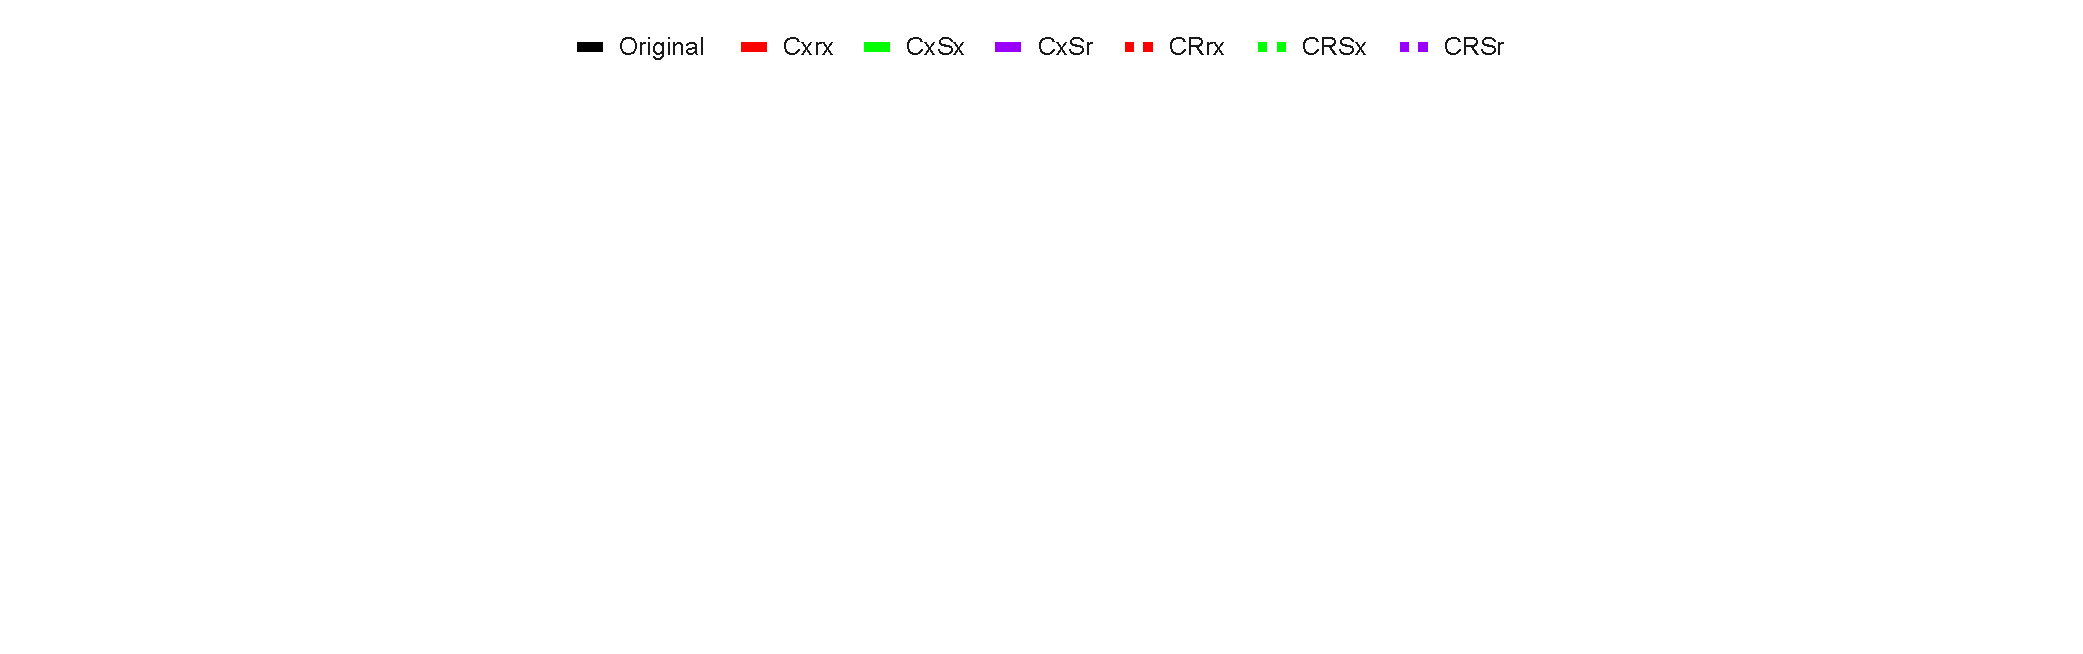
\includegraphics[width=0.98\linewidth]{out/im-key.pdf}
  } \\[-2ex]
  \subfigure{
    \label{fig:im-web-Stanford}
    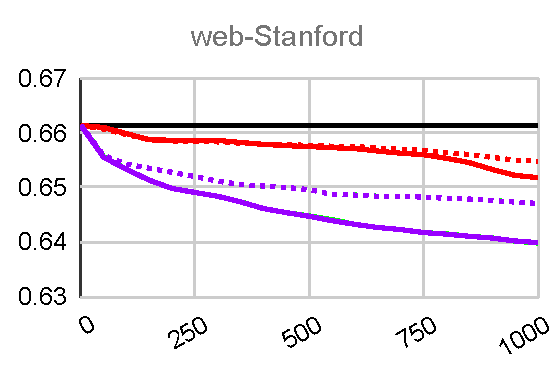
\includegraphics[width=0.23\linewidth]{out/im-web-Stanford.pdf}
  }
  \subfigure{
    \label{fig:im-web-BerkStan}
    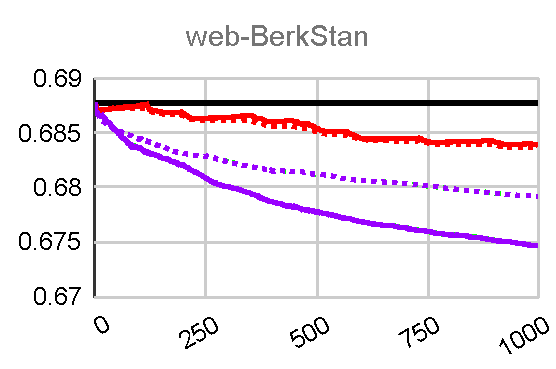
\includegraphics[width=0.23\linewidth]{out/im-web-BerkStan.pdf}
  }
  \subfigure{
    \label{fig:im-web-Google}
    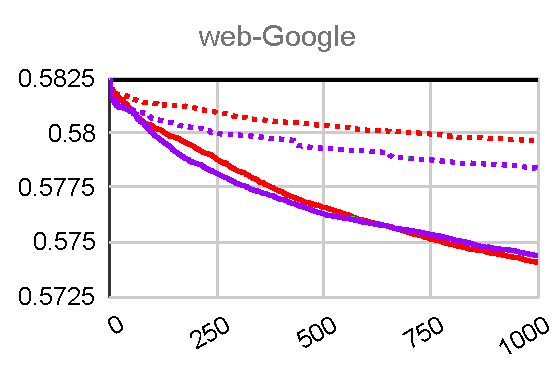
\includegraphics[width=0.23\linewidth]{out/im-web-Google.pdf}
  }
  \subfigure{
    \label{fig:im-web-NotreDame}
    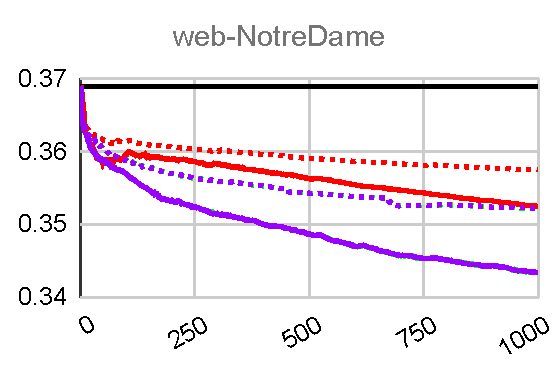
\includegraphics[width=0.23\linewidth]{out/im-web-NotreDame.pdf}
  }
  \subfigure{
    \label{fig:im-soc-Slashdot0811}
    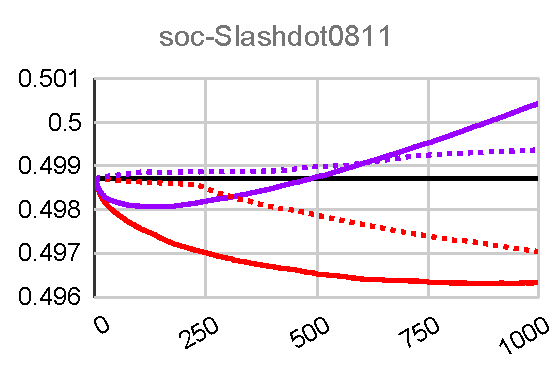
\includegraphics[width=0.23\linewidth]{out/im-soc-Slashdot0811.pdf}
  }
  \subfigure{
    \label{fig:im-soc-Slashdot0902}
    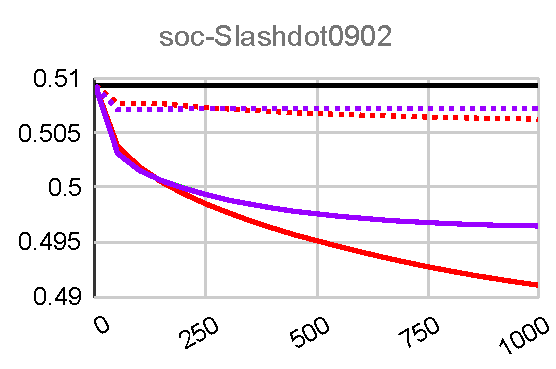
\includegraphics[width=0.23\linewidth]{out/im-soc-Slashdot0902.pdf}
  }
  \subfigure{
    \label{fig:im-soc-Epinions1}
    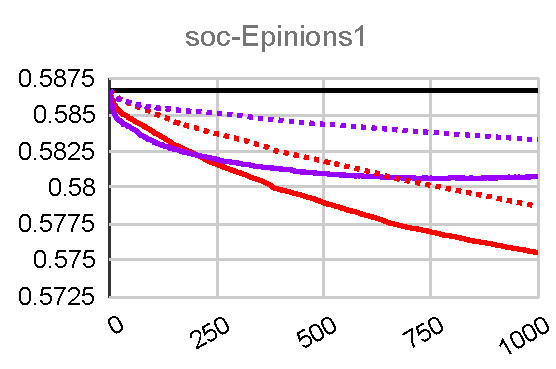
\includegraphics[width=0.23\linewidth]{out/im-soc-Epinions1.pdf}
  }
  \subfigure{
    \label{fig:im-soc-LiveJournal1}
    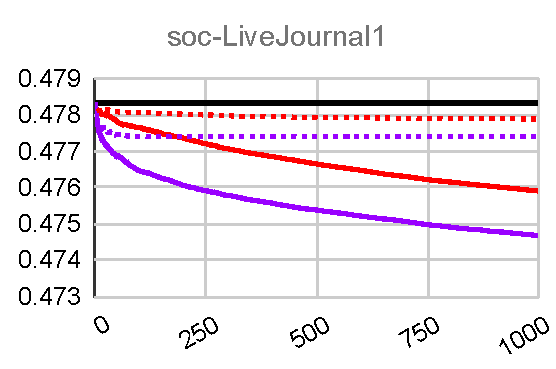
\includegraphics[width=0.23\linewidth]{out/im-soc-LiveJournal1.pdf}
  }
  \subfigure{
    \label{fig:im-coAuthorsDBLP}
    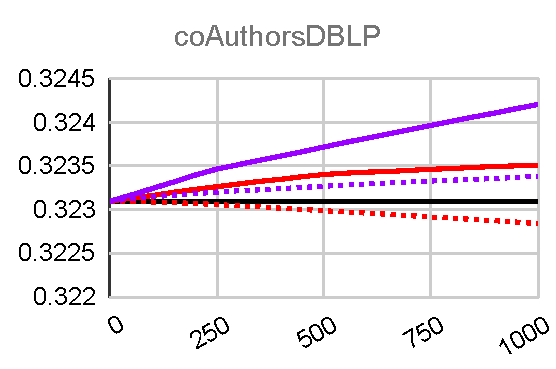
\includegraphics[width=0.23\linewidth]{out/im-coAuthorsDBLP.pdf}
  }
  \subfigure{
    \label{fig:im-coAuthorsCiteseer}
    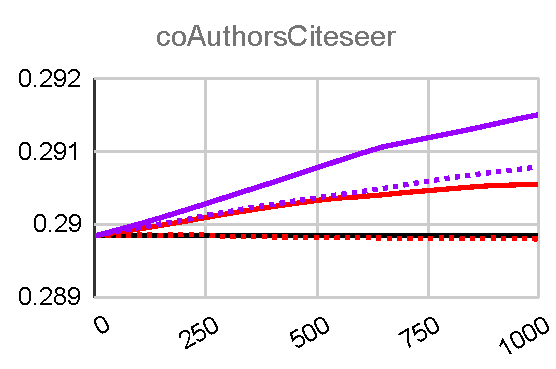
\includegraphics[width=0.23\linewidth]{out/im-coAuthorsCiteseer.pdf}
  }
  \subfigure{
    \label{fig:im-coPapersCiteseer}
    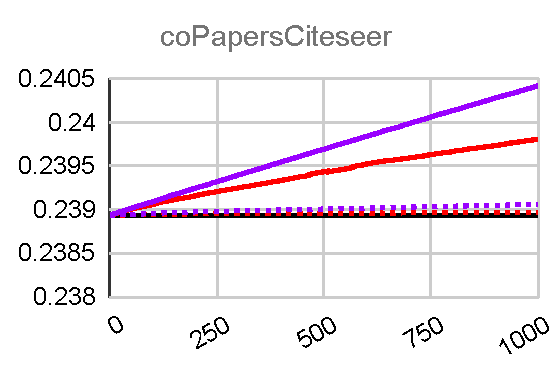
\includegraphics[width=0.23\linewidth]{out/im-coPapersCiteseer.pdf}
  }
  \subfigure{
    \label{fig:im-coPapersDBLP}
    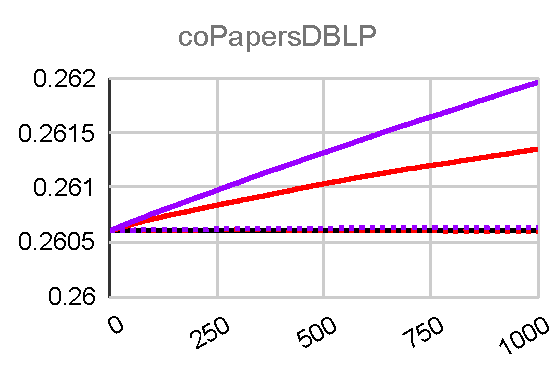
\includegraphics[width=0.23\linewidth]{out/im-coPapersDBLP.pdf}
  }
  \subfigure{
    \label{fig:im-italy_osm}
    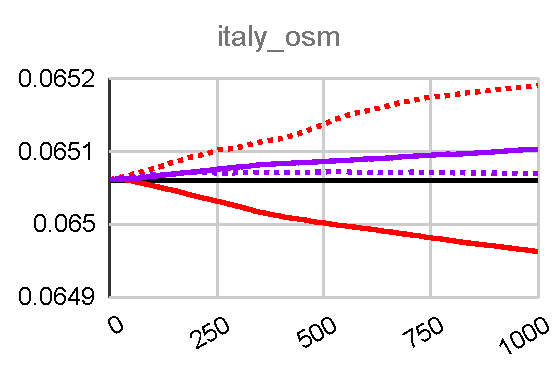
\includegraphics[width=0.23\linewidth]{out/im-italy_osm.pdf}
  }
  \subfigure{
    \label{fig:im-great-britain_osm}
    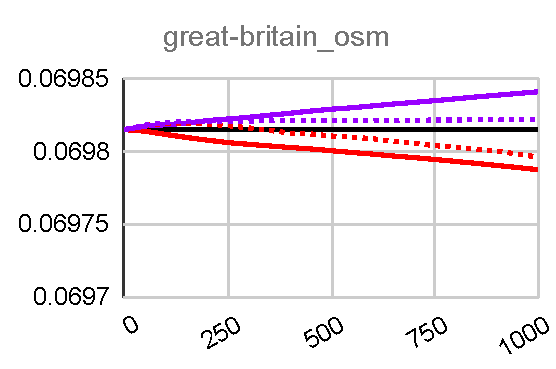
\includegraphics[width=0.23\linewidth]{out/im-great-britain_osm.pdf}
  }
  \subfigure{
    \label{fig:im-germany_osm}
    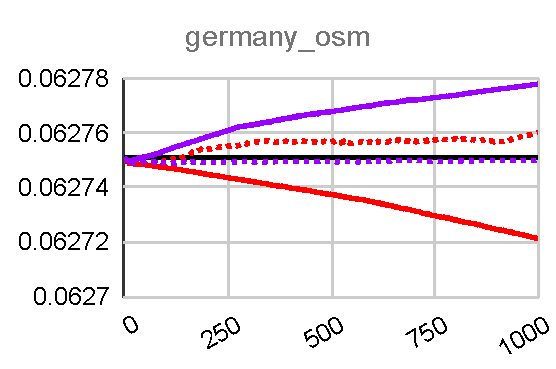
\includegraphics[width=0.23\linewidth]{out/im-germany_osm.pdf}
  }
  \subfigure{
    \label{fig:im-asia_osm}
    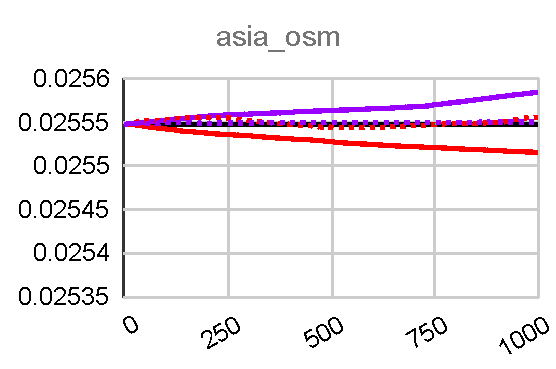
\includegraphics[width=0.23\linewidth]{out/im-asia_osm.pdf}
  }
  \subfigure{
    \label{fig:im-indochina-2004}
    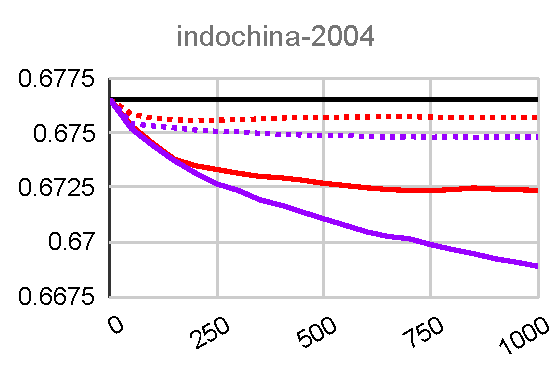
\includegraphics[width=0.23\linewidth]{out/im-indochina-2004.pdf}
  } \\[-2ex]
  \caption{Variation of Gini coefficient (Y-axis) with edges being added (X-axis) to the graphs incrementally with six different heuristics: \textit{edgeInsertCxrx}, \textit{edgeInsertCxSx}, \textit{edgeInsertCxSr}, \textit{edgeInsertCRrx}, \textit{edgeInsertCRSx}, and \textit{edgeInsertCRSr}.}
  \label{fig:im-all}
\end{figure*}



\section{Conclusion}
\label{sec:conclusion}
The study highlights that inequality is prevalent in web graphs, and demonstrates that efforts to minimize it are more effective in contexts with high Gini coefficients. The choice of heuristics plays a crucial role in reducing inequality. Our research suggests that a combination of \textbf{edgeInsertCxrx} and \textbf{edgeInsertCxSx} heuristics may offer an effective approach to minimize inequality. Future research should continue to explore strategies to mitigate inequality in web ranking algorithms and promote a more equitable web environment.


%% The acknowledgments section.
% \begin{acks}
% To my father, for the temple food and motivating a systematic workflow.
% \end{acks}

%% Bibliography style to be used, and the bibliography file.
\bibliographystyle{ACM-Reference-Format}
\bibliography{main}

\clearpage
\appendix
\section{Appendix}
\subsection{Gini coefficient of PageRank values with different dead-end handling strategies}

In this experiment we compare Gini coefficient of PageRank values obtained with three different dead-end handling strategies: \textit{teleport from dead-ends} (\textbf{Teleport}), \textit{self-loop dead-ends} (\textbf{Loop}), and \textit{self-loop all vertices} (\textbf{Loop-all}). This is measured for graphs given in Table \ref{tab:dataset}. The PageRank values of vertices in each graph is obtained with \href{https://www.npmjs.com/package/nvgraph.sh}{\textit{nvgraph.sh}} \cite{sahu2021nvgraph}, which internally uses \href{https://docs.nvidia.com/cuda/archive/10.0/nvgraph/index.html#nvgraph-pagerank-example}{\textit{nvGraph PageRank}} \cite{nvidia2018nvgraph}. The Lorenz curve of ranks is obtained by sorting the ranks in ascending order and cumulatively summing them up to obtain $100$ samples. These $100$ samples are then compared with the ideal (total equality) Lorenz curve to obtain the Gini coefficient.\ignore{Note that} This is output into YAML files by \textit{nvgraph.sh} itself. This measurement process of Lorenz curve and Gini coefficient is repeated for \textit{loop} and \textit{loopall} variants of graphs, which are generated from the original graph using \href{https://github.com/puzzlef/graph-generate}{\textit{graph-generate}} \cite{sahu2022github}. Finally we process all YAML files into CSV, separately for Gini coefficient and Lorenz curve, and compare the results.

\begin{figure*}[hbtp]
  \centering
  \subfigure{
    \label{fig:de-gini--mean}
    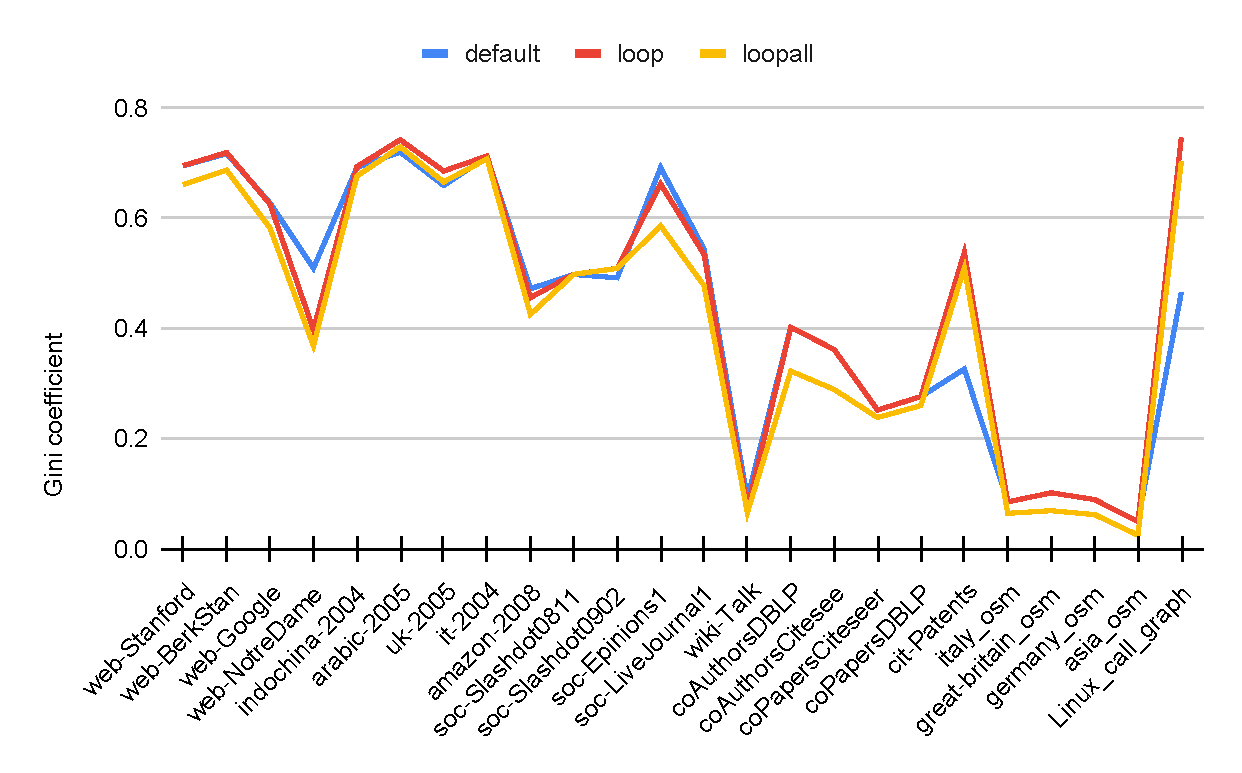
\includegraphics[width=0.68\linewidth]{out/de-gini.pdf}
  } \\[-2ex]
  \caption{Gini coefficient of PageRank values on 24 different graphs, comparing between PageRank values obtained with three different dead-end handling strategies: \textit{teleport from dead-ends} (\textbf{default}), \textit{self-loop dead-ends} (\textbf{loop}), and \textit{self-loop all vertices} (\textbf{loopall}).}
  \label{fig:de-gini}
\end{figure*}


\end{document}
\endinput
%% End of file.
